\documentclass[MIRU,submit]{miru2019j}
\usepackage{graphicx}
\usepackage{mathtools}
%\usepackage{latexsym}
%\usepackage[fleqn]{amsmath}
%\usepackage[psamsfonts]{amssymb}

\begin{document}

\title{レスキュー犬の一人称動画を用いた動作推定}

\affiliate{Tokyo}{電気通信大学 大学院情報理工学研究科 情報学専攻}
\affiliate{Tohoku}{東北大学NICHe}
\affiliate{rikei}{理研AIP}

 \author{荒木 勇人}{Tsuyohito ARAKI}{Tokyo}[araki-t@mm.inf.uec.ac.jp]
 \author{井出 佑汰}{Yuta IDE}{Tokyo}%[ide-y@mm.inf.uec.ac.jp]
 \author{濱田 龍之介}{Kazunori OHNO}{Tohoku}%[hamada@rm.is.tohoku.ac.jp]
 \author{大野 和則}{Kazunori OHNO}{Tohoku, rikei}%[]
 \author{柳井 啓司}{Keiji YANAI}{Tokyo}%[yanai@cs.uec.ac.jp]

% 概要・キーワードは省略して下さい.

\maketitle
\section*{概要}
被災地での災害救助を補助する犬をレスキュー(災害救助)犬といい,カメラなどの計測装置を装備したレスキュー犬をサイバーレスキュー犬と言う.
本研究では,犬にとりつけたセンサからサイバーレスキュー犬活動の識別を目的とする.
犬一人称動画像と音声をCNNを用いて動作毎に分類するsound/image-based three-stream CNNの提案と,提案手法をマルチクラス推定に用いた実験を行なった.
Sound/image-based three-stream CNNは動画から得られた静止画像・optical flow画像・音声を入力とする動画識別ネットワークである.
本提案手法の有効性を示すため,3つの入力それぞれ単体とその組み合わせパターン
(静止画像単体,optical flow画像単体,音声単体,静止画像+optical flow画像,静止画像+音声,optical flow画像+音声)
を用いた識別との比較実験を行なった.
結果は,51.8\%で提案手法で最も高い精度が得られた.
推定には,レスキュー犬の訓練の様子を撮影したデータセットを用いた.このデータセットは現在も作成中であり,まだ学習のデータ量が十分とは言えない.
一人称視点動画からのマルチクラス推定というタスクと,レスキュー犬訓練データセットの複雑さのあいまったチャレンジングなタスクであることを踏まえても不十分な結果であり,今後さらに手法の改良とデータセットの拡充が必要である.

\section{はじめに}
被災地での救助活動を行う際に,人間の補助として訓練されたレスキュー犬(災害救助犬)が探査を行う場合がある.
レスキュー犬は,犬としての特性を生かして人間と協力して被災地の探索を行う.
がれきの隙間などの狭い空間や倒壊した建物など人間には踏破困難な環境でも探査可能であり,発達した嗅覚を頼りにした救助活動が可能である.
しかし彼らは人間に向けた言語を持たないため,人間はレスキュー犬の行動から彼らが収集した情報を理解しなくてはならない.
現状では,レスキュー犬を指揮するハンドラーと呼ばれる人間がレスキュー犬の行動を手動でマーキングしており,その情報を消防などの指揮命令者に口頭伝達している.
このレスキュー犬との共同探索の問題点として,トリアージ(緊急度に従った手当の優先順位付け)のための周辺環境情報や,要救助者情報の不足があげられる.
また,ハンドラーによる記録はどうしても主観的になるので客観性に欠け,さらにそれが口頭伝達されることで正確性がより欠落する.
本研究では,レスキュー犬にセンサを装着して得られたデータを用いてレスキュー犬の行動推定を目的とする(図\ref{lite_model}).
本研究の具体的なタスクは, 映像だけでなく音声などのデータも活用したマルチモーダル情報を用いたクラス推定である.これにより,レスキュー犬が今何をしているのか個人の主観に基づくことなく判断することが可能となり,トリアージに必要な情報が整理され,災害救助活動の効率化が期待される.

\begin{figure}[tb]
 \begin{center}
%  \includegraphics[width=7cm]{./Figures/easy_image.eps}
  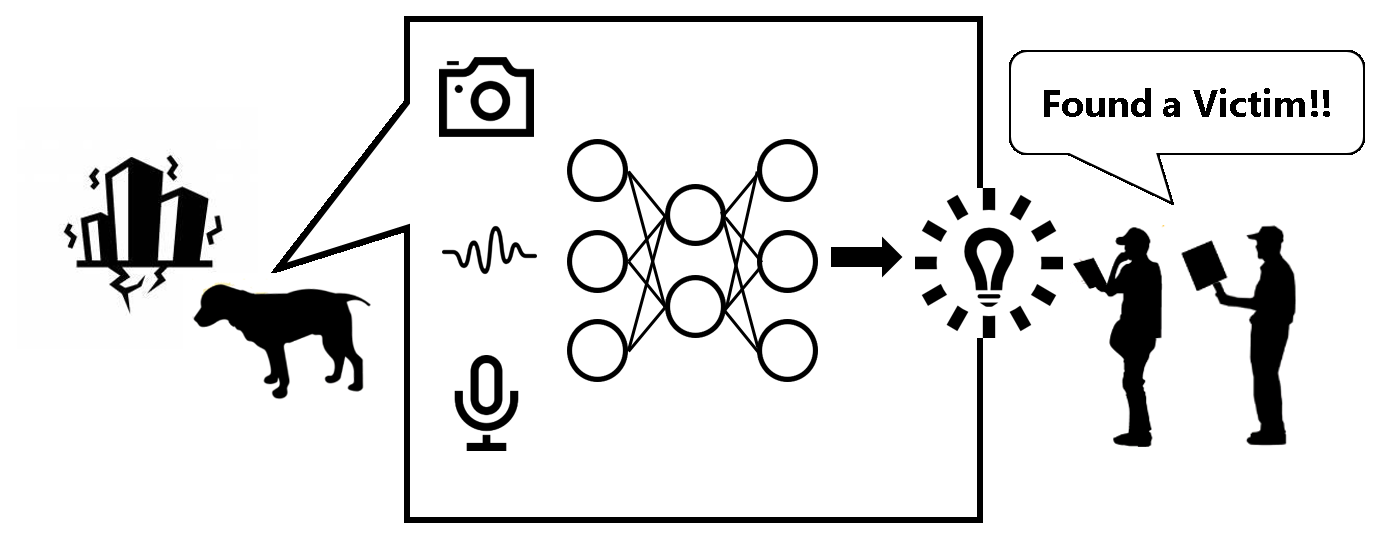
\includegraphics[width=7cm]{./Figures/dogactrec.eps}
  \caption{提案手法の概要.入力画像から複数データを抽出し,それぞれ別のストリームへ入力する.各ストリームの出力をもとに,動画のレスキュー犬行動推定結果を最終出力とする.}
  \label{lite_model}
 \end{center}
\end{figure}

\section{関連研究}
動画分類の研究に two-stream CNN ~\cite{simonyan2014two}がある.これは動画のフレームとフレームから求まる optical flow画像を個別のネットワークで学習することで動き情報を考慮した動画分類を行っている.

レスキュー犬行動のモニタリングのために,大野, 濱田らによって装着型計測・記録装置が開発された~\cite{dog01}.図~\ref{cyber}にレスキュー犬に装着可能な軽量な行動計測スーツを示す.これを着用したレスキュー犬はサイバー救助犬とも呼ばれる.各種センサを用いた計測データを記録し,リアルタイムに映像などのデータを無線配信することが可能である.そのため,レスキュー犬が人の目の及ばない範囲で活動する際にもレスキュー犬の行動やその周辺環境などを把握するのに役立つ.

また,Ehsanらによる犬の一人称視点動画からの犬行動予測の研究がある~\cite{whoretthedog}.これは,犬の行動をモデリングし,犬が次にどのような道をたどり行動するかを予測している.

しかし,これらの研究は犬の行動のモデリングであり,犬の周辺環境の推定などは行っていない.また,入力は動画像のみであり,音声などのデータは利用していない.レスキュー犬の課題には,犬の周辺環境情報や動画像からだけでは判断できない情報の取得が含まれている.例えばレスキュー犬は要救助者を発見するとその場で待機し吠え続けるように訓練されている.
このように,動画像データからだけではなく,音声データ,および慣性データ・GPSデータなどの情報を複合的に用いてレスキュー犬の状態を判断しなければならない.
ただし, 本研究では動画像と音声情報のみの提供をうけたため, これらを入力とした犬の行動推定を行う.

音声に焦点をあてた動画分類の研究にはSoundNet~\cite{aytar2016soundnet}がある.
動画から音声と画像を取り出し,画像を教師データとし,音声は生徒データとして出力が等しくなるように学習している.
この手法は音響シーン分類,物体分類の標準ベンチマークにおいて教師あり学習の最高精度を達成した.
本研究では音声のみからの行動推定は目的としない.しかし,音声の意味的情報は動画認識に重要であることが明らかにされている.
SoundNetとtwo-stream CNN を参考に, 本研究では音声識別ネットワークと two-streamネットワークを統合したアーキテクチャを構築した.
SoundNetが音声波形を入力とするのに対し,本研究では音声からMFCC特徴を抽出してからストリームへの入力とする点で異なっている.

音声と動画像だけでなく,加速度と速度情報を用いたマルチモーダルな学習の研究には丹野らの~\cite{tanno2019deim}がある.
これは,情報を追加することによっての認識精度の向上や低下を報告しており,特に音声によって分類精度が向上するとされている.
マルチモーダルな深層学習という点で本研究と同様のテーマだが,マルチクラス推定という点で本研究とは異なっている.

\begin{figure}[tb]
 \begin{center}
  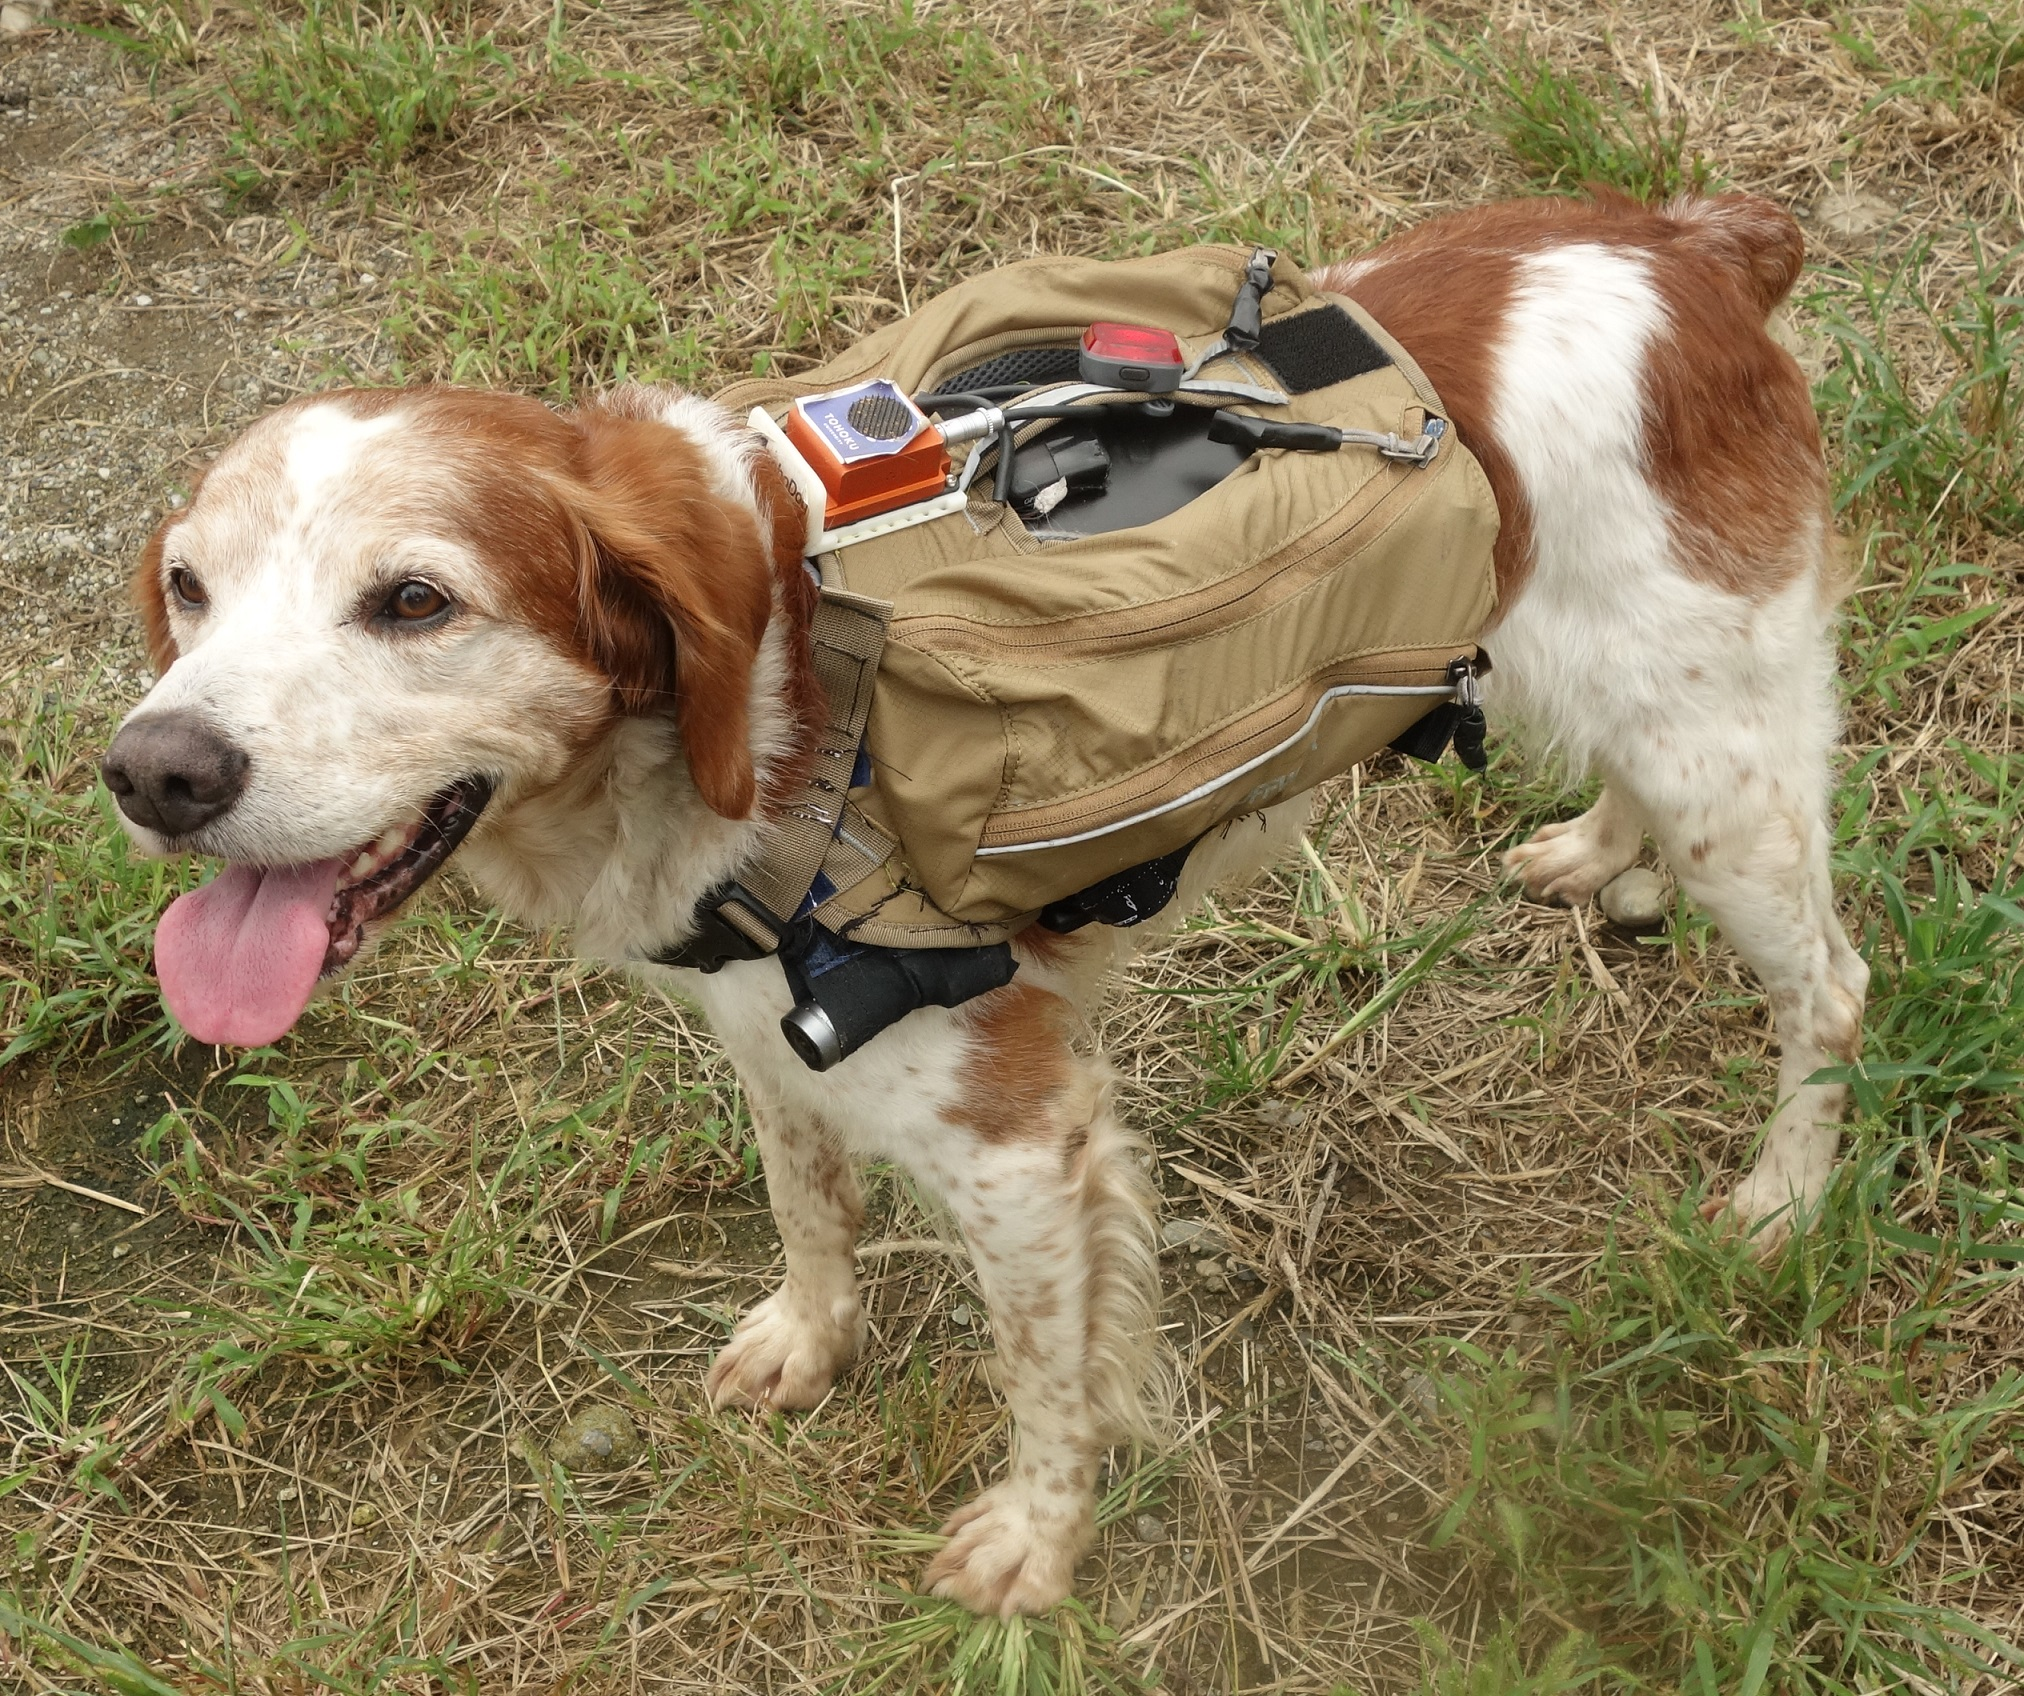
\includegraphics[width=5cm]{./Figures/cyberdog.eps}
  \caption{装着型計測・記録装置~\cite{dog01}より引用.}
  \label{cyber}
 \end{center}
\end{figure}

\section{データセット}
学習には,サイバーレスキュー犬訓練データセットを利用した.これは,訓練されているレスキュー犬に専用の計測スーツを着用させ収集したデータ群である.東北大学の大野らからその一部を提供された.
提供されたデータは7本からなる動画で, 時間の範囲を指定するように犬行動がラベル付けされている.
犬行動は11種(bark:吠える, cling:匂いに執着する, command:ハンドラーからの働きかけがある, eat-drink:飲食する, look\_at\_handler:ハンドラーを見る, run:走る, see\_victim:要救助者を発見した, shake:体をブルブルと震わせる, sniff:匂いを嗅ぐ, stop:脚を止める, walk-trot:歩く)あり, その一部を図~\ref{dataset}に示す.
総時間は57分40秒,秒間フレーム数は29.97,総フレーム数は103,696枚である.
分類クラスそれぞれについて時間範囲を指定する形で動画にアノテーションがされており,同時刻に複数のクラスが重なるためマルチラベルデータとして取り扱う.
これを 6fpsにサンプリングして整形したものを学習と評価に用いた.クラス毎の出現頻度が~表\ref{cyberdataset_label}の値である.表記のためクラス名を簡略した.
各クラス毎に約100回から9000回のサンプルがあり数値上では十分である.
しかしこれは連続したシーンを含めての数値であり,その実は多様性に欠ける中身となっている.
例えば,runクラスは98サンプルあるが,独立したシーンとしては3シーンにすぎず,
bark,eat-drink,see\_victim,shakeクラスを合わせても100シーンに満たない.

\begin{table*}[htb]
 \begin{center}
 \caption{サイバーレスキュー犬訓練データセット 利用範囲内で計測した出現回数}\label{cyberdataset_label}
 \scalebox{0.95}[0.95]{
  \begin{tabular}{|l||c|c|c|c|c|c|c|c|c|c|c|}
   \hline \hline
      クラス   & \rotatebox{90}{bark}& \rotatebox{90}{cling}&\rotatebox{90}{command}& \rotatebox{90}{eat}&\rotatebox{90}{handler}& \rotatebox{90}{run}&\rotatebox{90}{victim}& \rotatebox{90}{shake}& \rotatebox{90}{sniff}& \rotatebox{90}{stop}& \rotatebox{90}{walk} \\ \hline

%   ラベル & bark&cling&comm&eat&handler&run&victim&shake&sniff&stop&walk \\ \hline
   出現回数& 1744& 1127&2439&343&  2011& 98&  1549&  239& 7719&6384&8764 \\ \hline
  \end{tabular}
 }
\end{center}
\end{table*}

フレームの静止画像とその直後のフレームから計算したoptical flow画像, および前後15フレーム分の長さの音声の3データをフレーム毎に抽出した.

%これを1/5の量にサンプリングしたものを学習と評価に用いた.

\begin{figure}[tb]
    \begin{tabular}{l}

      \begin{minipage}{0.32\hsize}
        \begin{center}
          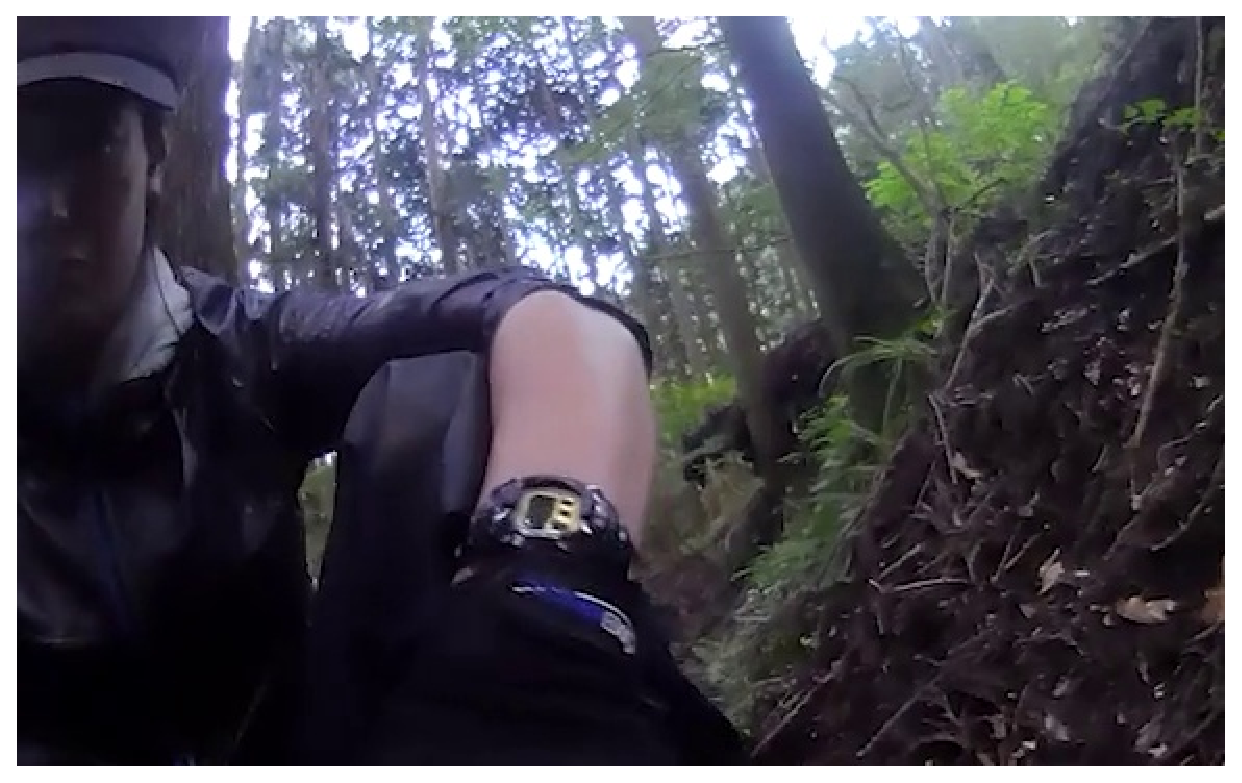
\includegraphics[clip, width=2.8cm]{./Figures/still_seevictim3.eps}
        \end{center}
      \end{minipage}

      \begin{minipage}{0.32\hsize}
        \begin{center}
          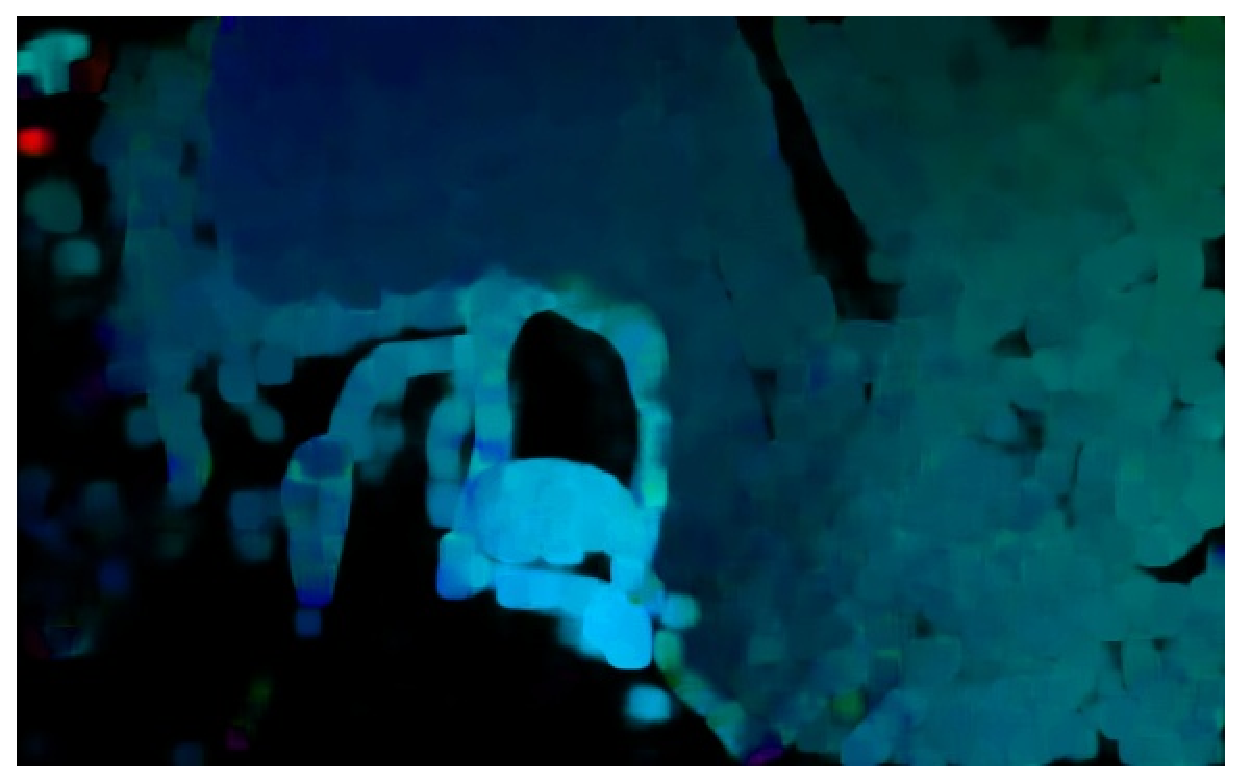
\includegraphics[clip, width=2.8cm]{./Figures/optic_seevictim3.eps}
           %\hspace{2.0cm} {}
        \end{center}
      \end{minipage}

      \begin{minipage}{0.32\hsize}
        \begin{center}
          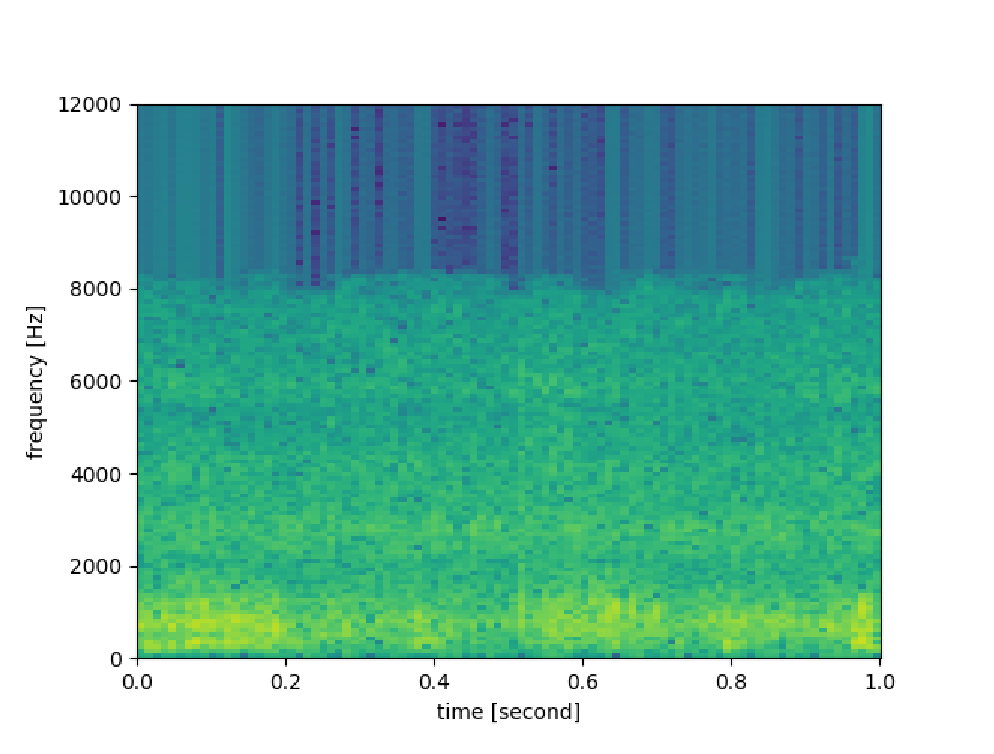
\includegraphics[clip, width=2.8cm]{./Figures/sound_seevictim.eps}
        \end{center}
      \end{minipage}
%    \end{tabular}
\\  %%%%%%%%%%%%%%%%
      \begin{minipage}{0.32\hsize}
        \begin{center}
          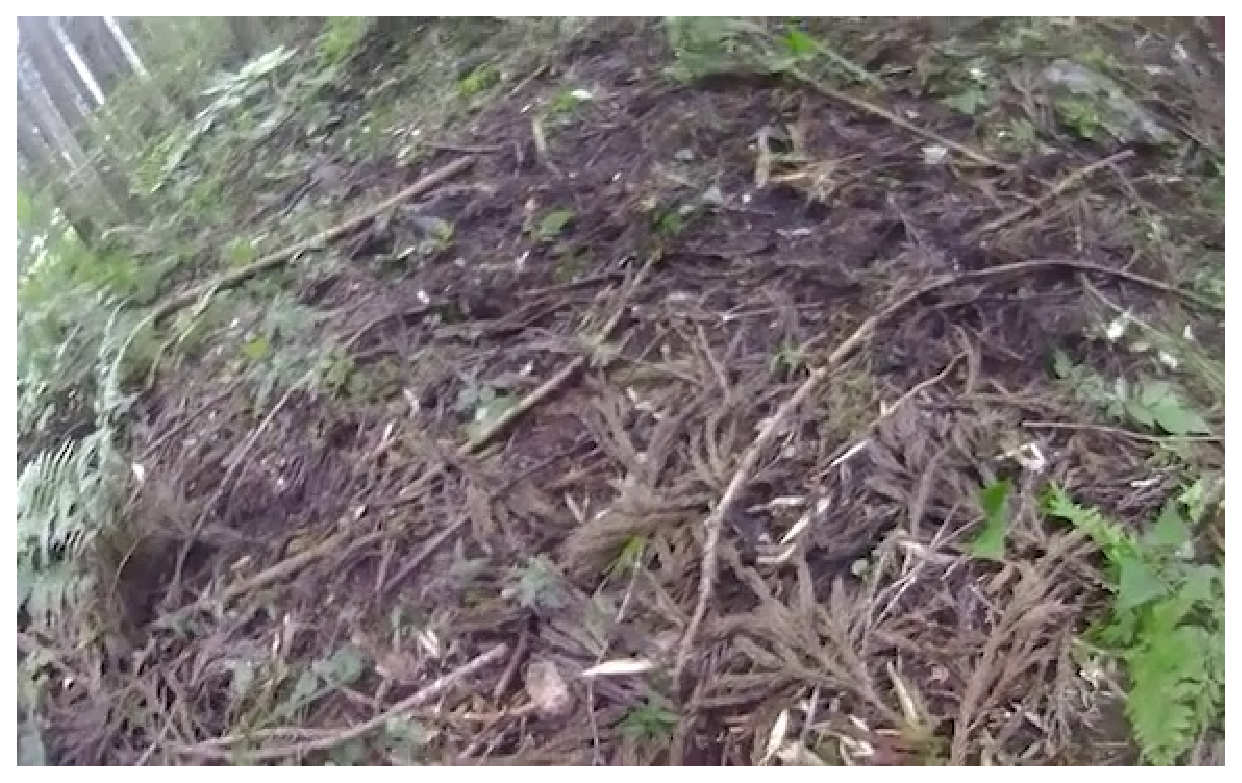
\includegraphics[clip, width=2.8cm]{./Figures/still_stop1-3.eps}
        \end{center}
      \end{minipage}
      \begin{minipage}{0.32\hsize}
        \begin{center}
          
\includegraphics[clip, width=2.8cm]{./Figures/optic_stop1-3.eps}
        \end{center}
      \end{minipage}
      \begin{minipage}{0.32\hsize}
        \begin{center}
          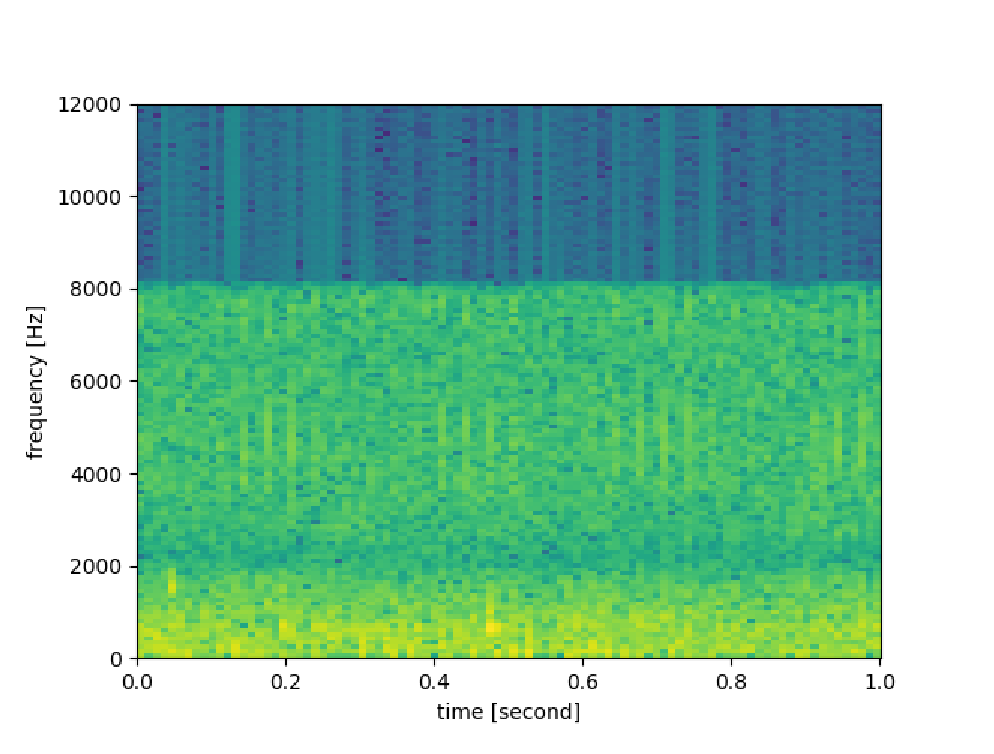
\includegraphics[clip, width=2.8cm]{./Figures/sound_stop2.eps}
        \end{center}
      \end{minipage}
    \end{tabular}
    \caption{サイバーレスキュー犬訓練データセットsee victimクラス(上段)とstopクラス(下段). 左から静止画像, optical flow画像, MFCCスペクトラムで可視化した音声である.}
    \label{dataset}
\end{figure}


\section{提案手法}
本研究ではレスキュー犬の行動推定のために,動画像・音声のマルチラベル推定を行う.
そのため,レスキュー犬訓練データセットを認識するためのsound/image-based three-stream CNNを提案する.
これは,two-stream CNN に音声ストリームを加えたモデルである.静止画像, optical flow画像, 音声を別々のストリームへの入力とし,それぞれの出力を元にレスキュー犬の行動を推定する.
Sound/image-based three-stream CNN のアーキテクチャを図~\ref{sound3st}に示す.

まず入力となる動画から静止画像のフレーム($F_t$)を取り出し,直後の$F_{t+1}$間とのoptical flow画像($O_t$)を生成する.次に両画像から同じ構造の2つのネットワークを用いて特徴量の抽出を行う.
そして対応する音声($A_t$)からMFCC($M_t$)を求め,前述とは異なる構造のネットワークを用いて($M_t$)から特徴量の抽出を行う.
最後にこれら2つあるいは3つの特徴量の組み合わせ毎に結合し,分類ネットワークでクラス分類を行う.
この際に,音声をフレームと同じサイズで切り出すと特徴が著しく失われるため入力音声には$F_t$の前後0.5秒ずつを用いた.動画あるいは音声から実際に犬の行動を推定する場合を想定し,現実的で取り扱いやすい時間としてこれを設定した.
動画長は31フレームとし,中央から切り出した静止画像とそれに対応する直後のoptical flow画像をそれぞれImageNetで学習済みのVGG16モデルに通し,畳み込み層の出力を結合した.
動画から切り出した音声は畳み込みを繰り返すと特徴の縦横次元が小さくなるため,静止画像の畳み込みの出力と同じサイズになるように調整した.
調整は畳み込みで奥行き次元を揃えた後,同じ特徴をリピートし目的の大きさになるまでコピーして結合した.
分類はフレーム毎に行った.
推定にはクラス毎にSoftMarginLossを用いた.
入力を$x$,出力を$y$,クラス数を$C$とすると,マルチクラス推定の損失関数SoftMarginLossは式~\ref{softmargin}に定義される.
推定クラスが正解なら$\Sigma$内の第2項,不正解なら第1項が計算に利用するように設計されており,推定ラベルによって関数が変わる.
本研究では11クラスを取り扱うため,出力yは11次元のバイナリとする.
閾値=0.5とし,閾値以上のクラスを推定クラスとした.
\begin{equation}
    \label{softmargin}
    \begin{split}
    loss(x, y) = &-\frac{1}{C} * \Sigma_{i} \{y[i]\} * log((1+exp(-x[i]))^{-1}])\\
    &+ (1 - y[i]) * log(\frac{exp(-x[i])}{1+exp(-x[i])})
    \end{split}
\end{equation}

学習は全てにおいて100エポック行った.学習率は1e-03〜1e-06,バッチサイズは32〜128の範囲で学習毎に変え制限の中で最も良い精度の結果を評価した.

\begin{figure}[tb]
   \begin{center}
    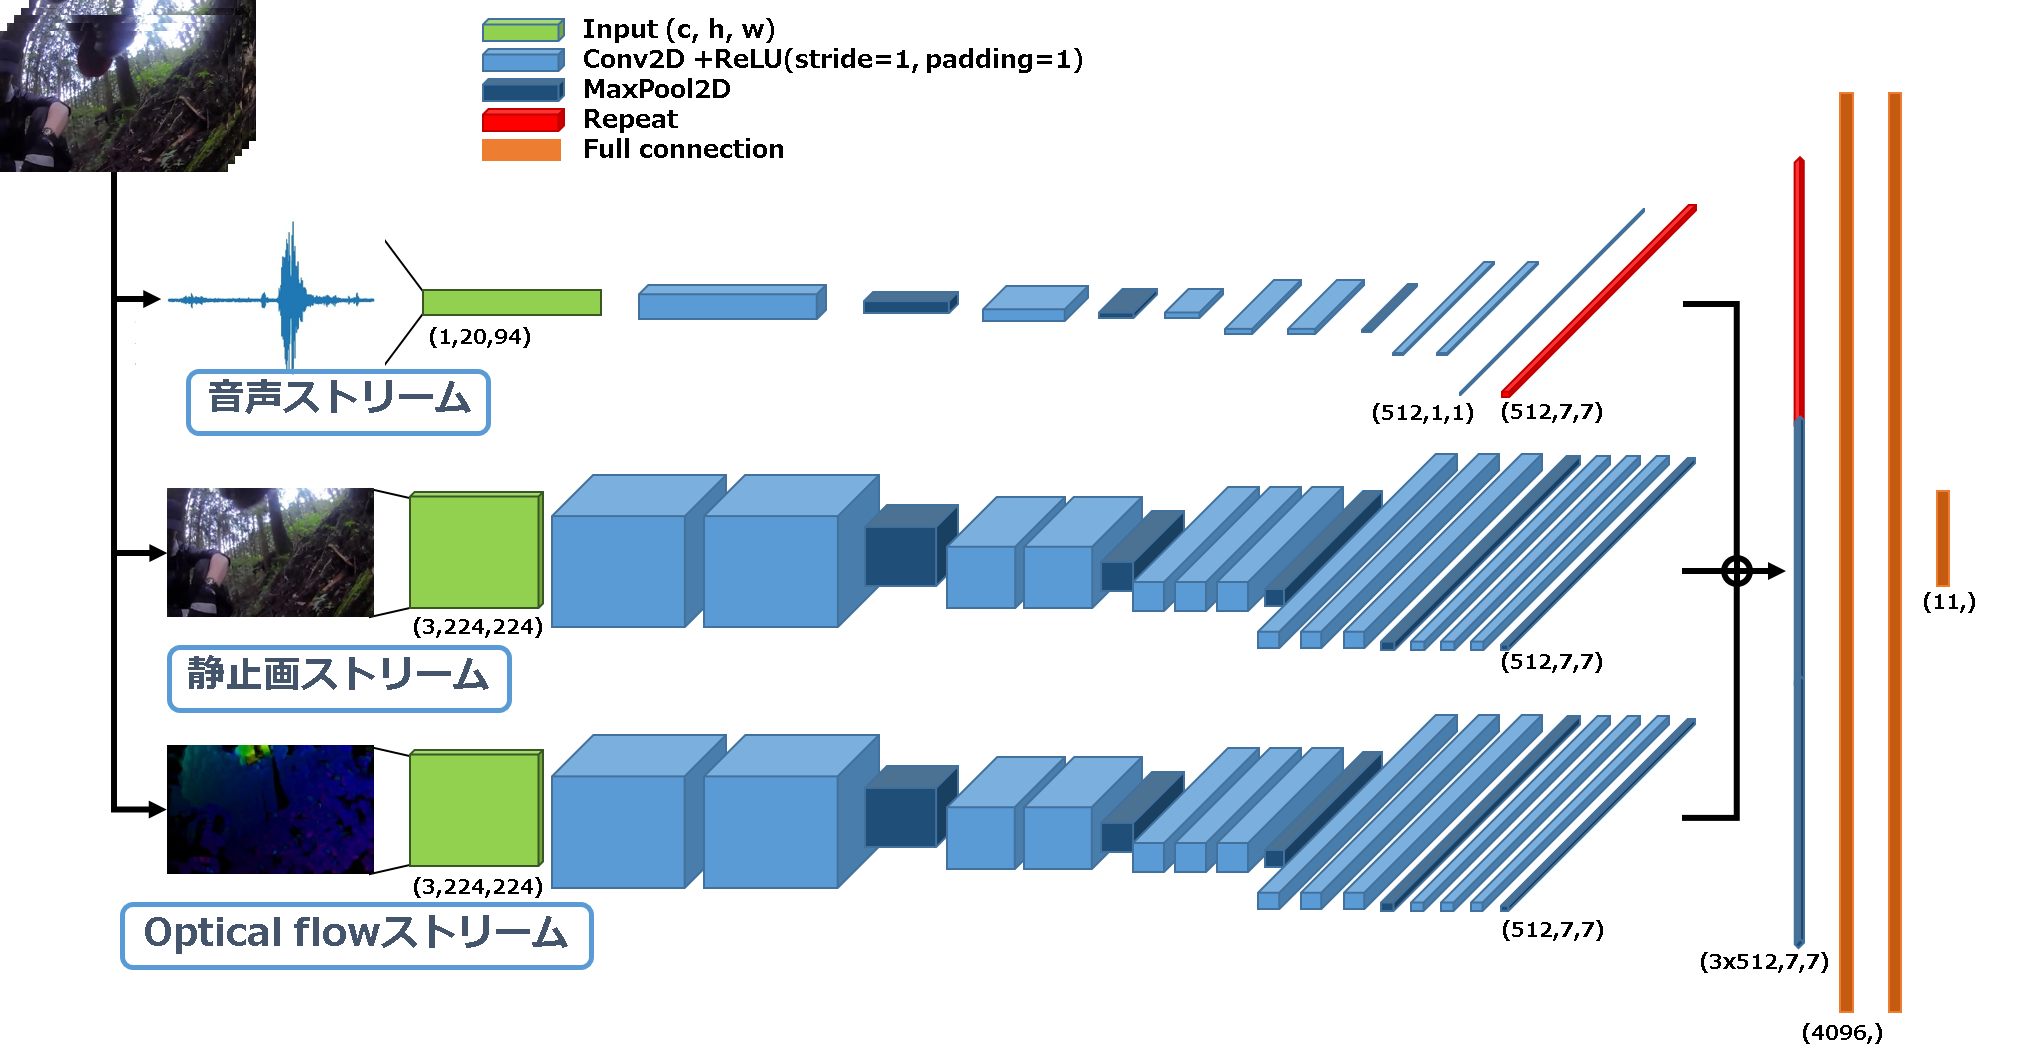
\includegraphics[scale=0.25]{./Figures/soundimage-basedthree-streamCNN.eps}
    \caption{Sound/image-based three-streamアーキテクチャ.音声, 静止画像, optical flow画像それぞれを入力とする3ストリームからなり, それぞれの出力を結合してクラスを推定している.}
    \label{sound3st}
   \end{center}
\end{figure}

\section{実験}

3つの入力について, それぞれ単体, 2つずつの組み合わせおよび全てを統合した場合の8通りを行った.%(表~\ref{ablation}).
画像単体を入力とした実験ではImageNetを学習したVGG16の学習済みモデルを用い再学習した.
音声での学習は畳み込み層について1Dと2Dの2種類で行った.
畳み込み層の次元の差について図~\ref{1d2dconv}に詳細を示す.出力の向きを合わせるために, 提案手法の複数入力には2Dの畳み込みを用いた.
一人称視点動画像からのマルチ行動推定を行なった先行研究は見つけられなかったため,既存手法との比較は行なっていない.
表では,クラス毎の精度と全体を合計しての精度をJaccard係数で示している.
なお,Jaccard係数とは$$\frac{TP}{FP+FN+TP}$$で表され,PrecisionとRecallの両者についてF尺度と比較してより厳格な値が求まる.
レスキュー犬の行動分類にあたり,PrecisionとRecallを共に重視するためにこの係数を採用した.
よって,本研究ではJaccard係数がより大きいモデルは精度がより良いと表現する.

結果のまとめを表~\ref{expetiments_result}に示す.
静止画像, optical flow画像単体では精度が低く, これらを組合せたもので精度が上昇した.
比較して, 音声単体では1D, 2Dともに精度が高かった.音声と静止画像,音声とoptical flow画像を組合せた実験では,音声単体と比較して全体的な精度は低下した.
しかし,静止画像, optical flow画像, 音声の3つを組合せた提案手法では全体的な精度の上昇が見られ, クラス別で見ても半数以上のクラスの数値が上昇している.
人間が耳で聞いた際にもその特徴を識別しやすいbark, shakeクラスにおいては音声単体を1D畳み込み層で学習したものの方が数値が高い.
これらから, データセットに対する提案手法の有効性が示された.

\begin{figure}[tb]
   \begin{center}
    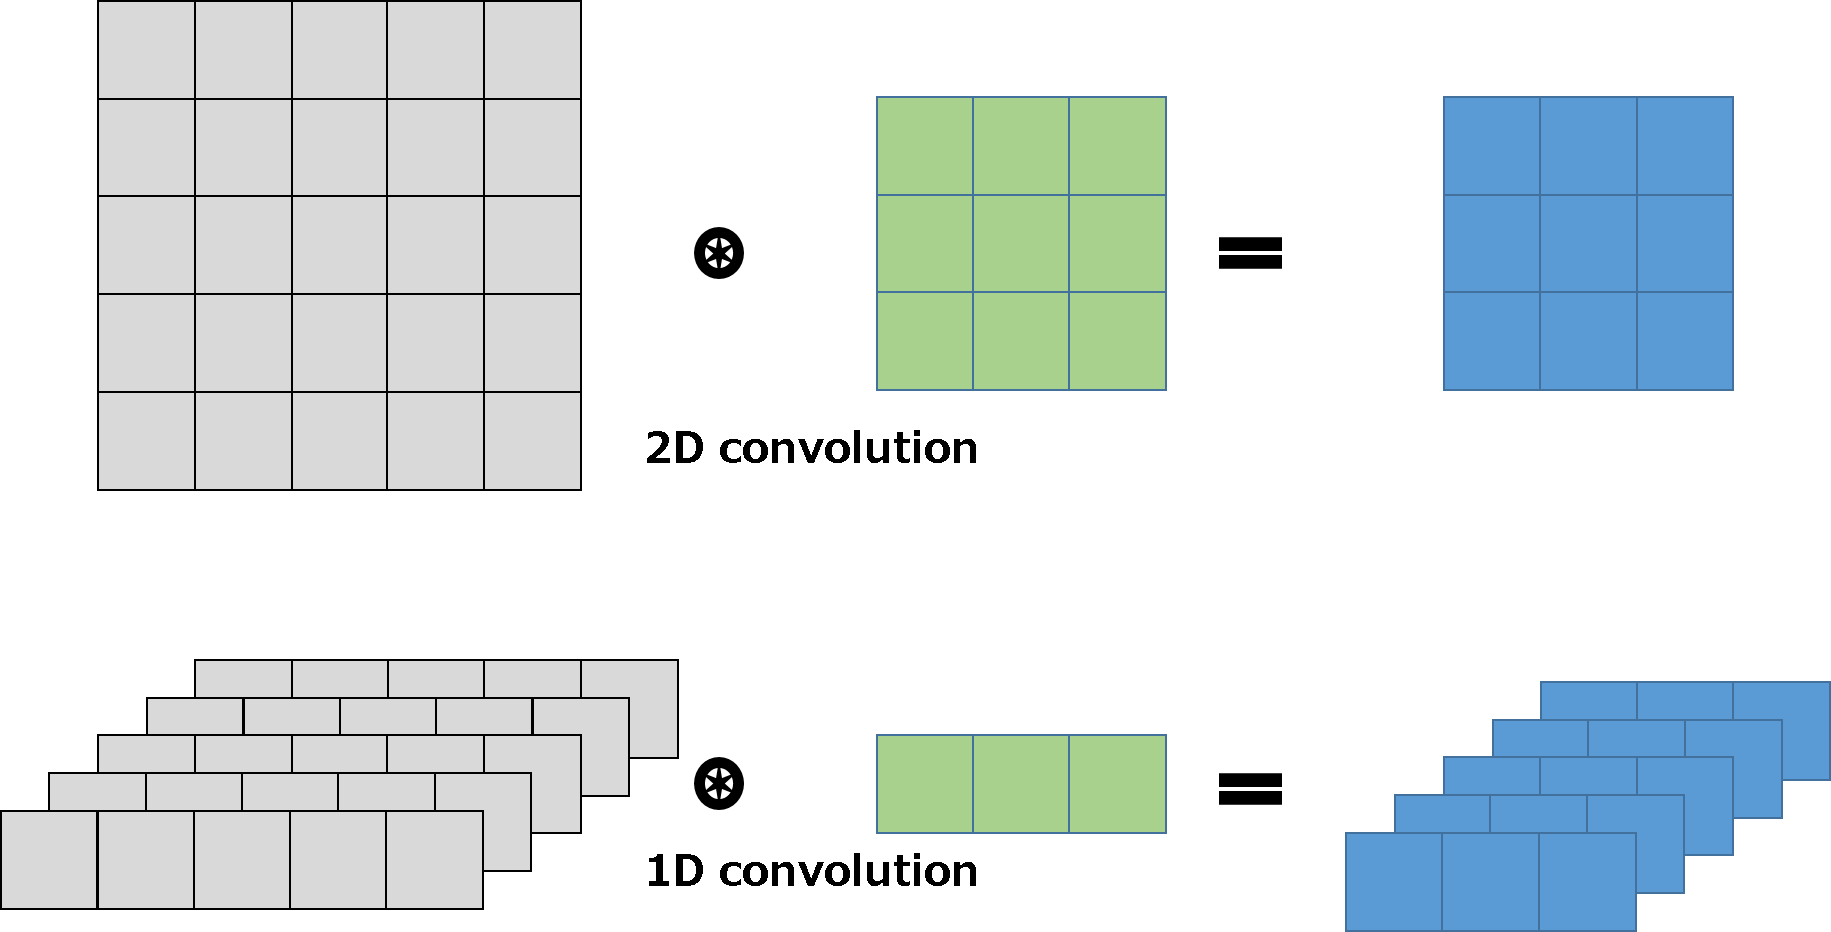
\includegraphics[scale=0.16]{./Figures/1d2dconv.eps}
    \caption{1D convolutionと 2D convolutionの詳細.データは同様でも入力の形と処理が異なり, 出力の結果も異なっている.}
    \label{1d2dconv}
   \end{center}
\end{figure}

\begin{table*}[htb]
% \centering
 \begin{center}
 \caption{各実験結果比較表.}\label{expetiments_result}
 \scalebox{0.85}[0.85]{
  \begin{tabular}{|l|c|c|c||c|c|c|c|c|c|c|c|c|c|c|c|}
   \hline \hline
   &静止画像&optical flow画像&音声& \rotatebox{90}{bark}& \rotatebox{90}{cling}&\rotatebox{90}{command}& \rotatebox{90}{eat}&\rotatebox{90}{handler}& \rotatebox{90}{run}&\rotatebox{90}{victim}& \rotatebox{90}{shake}& \rotatebox{90}{sniff}& \rotatebox{90}{stop}& \rotatebox{90}{walk} & \rotatebox{90}{全体}\\ \hline \hline
(1) & ◯ & × & ×  & 0.244& 0.066& 0.0& 0.024& 0.057& 0.0& 0.204& 0.0& 0.0& 0.588& 0.51&  0.436 \\ \hline
(2) & × & ◯ & ×  & 0.141& 0.0& 0.0& 0.0& 0.017& 0.0& 0.017& 0.0& 0.0& 0.586& 0.476&  0.406 \\ \hline
(3) & × & ×  &1D  & {\bf 0.669}& 0.078& 0.22& 0.023& 0.138& 0.0& 0.274& {\bf 0.44}& 0.502& 0.745& 0.704&  0.512 \\ \hline
(4) & × & ×  &2D  & 0.563& 0.04& 0.188& 0.001& 0.059& 0.0& 0.201& 0.304& 0.524& 0.744& {\bf 0.74}&  0.512 \\ \hline
(5) & ◯ & ◯ & × & 0.11& 0.018& 0.043& 0.0& 0.155& 0.0& 0.259& 0.0& 0.426& 0.705& 0.668&  0.435 \\ \hline
(6) & ◯ & × &2D & 0.662& 0.031& 0.195& 0.018& 0.115& 0.002& 0.308& 0.402& 0.498& 0.726& 0.694&  0.5 \\ \hline
(7) & × & ◯ &2D & 0.667& 0.054& {\bf 0.234}& 0.014& 0.123& 0.01& 0.223& 0.356& 0.487& 0.759& 0.692&  0.493 \\ \hline
(8) & ◯ & ◯ &2D & 0.577& {\bf 0.135}& 0.186& {\bf 0.066}& {\bf 0.183}& {\bf 0.026}& {\bf 0.433}& 0.409& {\bf 0.53}& {\bf 0.779}& 0.725 & {\bf 0.518} \\ \hline
  \end{tabular}
 }


 \end{center}
\end{table*}


\section{考察}
Sound/image-based three-stream CNNの提案と, 提案手法を用いたレスキュー犬の行動推定を行なった.
音声データはクラス推定に強力であるものの,音声・静止画像・optical flow画像の3つのデータにそれぞれ必要な情報が含まれていることがわかった.
提案手法が相対的に最も精度が高かったが, 51.8\%と数値では決して高いとは言えない.
本研究の目的はレスキュー犬の行動推定という人命のかかったタスクである.ハンドラーの補助的な役割を任せた運用をこなせるとしても,実際に現場で判断を任せるにはまだまだ不十分な結果となった.

精度をより上げるためには, 現在の手法の改良, 新しい手法の取り入れ, データセットの拡張が考えられる.
例えば, 音声について現在は静止画像の前後1秒を抽出しているが最適なフレーム長を調べるなどの余地がある.
特徴抽出についても今回は音声の特徴抽出にMFCC特徴を採用したが,\cite{aytar2016soundnet}のように波形をそのまま入力する分類手法も存在する.
また, 人間の一人称視点映像の分類研究で用いられているような動画分類特有の処理を入れるなどの手法を取り入れることで精度の向上が期待できる.
例えば,\cite{minghuang2016fpar}で用いられている腕のセグメンテーションネットワークのように,犬領域を推定するようなネットワークは犬動作の推定にも応用できる.
これは犬の状態推定への貢献が期待される.
ただし,腕領域とは異なり犬領域のデータセットは確認できていない.
音声からの特徴抽出は,音声フレームの長さが実験に対して適しているのかという疑問も残っている.
今回は検証しなかったが,本来は推定に最適なフレーム長を求めるべきである.
より適切な音声フレーム長が判断できればより高い精度も期待できる.
音声の特徴抽出方法についても最適と断言するには至っていない.今回音声の特徴抽出にMFCCを採用したが,\cite{aytar2016soundnet}のように波形をそのまま入力する分類手法も存在する.今回は取り扱わなかったが,検討の価値があるだろう.
データセットについても本研究で利用した内容は十分ではない.特に,eat, shake, runクラスなどは圧倒的にデータ量が少ない.
クラス毎のデータ数だけでなく, 慣性センサなどから取得される情報の利用も動作推定の精度向上に対する効果が期待される.レスキュー犬訓練データの増強は必須課題とも言える.

さらに,今回は研究の範囲としなかったが実際の現場での利用を想定した場合,レスキュー犬行動動画の入力に対してリアルタイムに結果を出すことも求められる.

\bibliographystyle{miru2019j}
\bibliography{ref}

% \begin{thebibliography}{9}% 文献数が10未満の時 {9}
% \bibitem{1}
% W. Rice, A. C. Wine, and B. D. Grain,
% diffusion of impurities during epitaxy,
% Proc. IEEE, vol.~52, no.~3, pp.~284--290, March 1964.
% \bibitem{2}
%  H. Tong, Nonlinear Time Series: A Dynamical System Approach, J. B. Elsner, ed., Oxford University Press, Oxford, 1990.
% \bibitem{3}
% H. K. Hartline, A. B. Smith, and F. Ratlliff,
% Inhibitoryinteraction in the retina,
% in Handbook of Sensory Physiology,
% ed. M. G. F. Fuortes, pp.~381--390, Springer-Verlag, Berlin.
% \bibitem{4}
% Y. Yamamoto, S. Machida, and K. Igeta,
% ``Micro-cavity semiconductors with enhanced spontaneous emission,''
% Proc. 16th European Conf. on Opt. Commun.,
% no.~MoF4.6, pp.~3--13, Amsterdam, The Netherlands, Sept.1990.
% \end{thebibliography}

\end{document}
